\chapter{Problemi insolubili} \label{ch:capitolo4}
\subsection{La macchina di turing Universale}
\textbf{Teorema}\\
La funzione g : $N^2 \mapsto N$ definita ponendo, per ogni x , y $\in$ $N$
\begin{center}
    g(x,y) = $\phi_x$(y)
\end{center}
è calcolabile secondo turing.\\\\
\textbf{Dimostrazione}
Su un input (x,y) $\in$ $N^2$
\begin{enumerate}
    \item Decodifica le istruzioni di M$_x$
    
    \item Simula M$_x$ sull’input y
    
    \item Se M$_x$ si arresta, restituisci l’output della computazione
\end{enumerate}
\textbf{Definizione}\\
La macchina di Turing $\mu$ che calcola la funzione g si dice Macchina di Turing universale.\\
La macchina di Turing universale ha la capacità di eseguire qualunque algoritmo.\\
Calcolatore all purpose (modello di Von Neumann).
\newpage
\subsection{La diagonalizzazione}
\textbf{Teorema}
L'insieme $R$ non è numerabile.\\\\
\textbf{Dimostrazione}\\
Per assurdo. Se $R$ fosse numerabile, avremmo una tabella infinita con tutti i numeri reali:\\
\begin{figure}[htp]
    \centering
    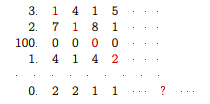
\includegraphics[scale=0.8]{tesi_stile/img/diagonalizzazione.png}
\end{figure}\\
Costruiamo un numero reale x = 0,c$_1$,c$_2$,c$_3$ ... in cui la i-esima cifra decimale è diversa dalla i-esima cifra rossa (e anche da 0 e 9).\\
Per esempio: 0.2211 ...\\
Dove può comparire nella nostra tabella?
\newpage
\subsection{Il problema dell'arresto}
Data una macchina di Turing M e un input y, decidere se M si arresta sull’input y.\\
\begin{center}
    H = \{(x,y) $\in$ $N^2$ $|$ M$_x$ $\downarrow$ y\}
\end{center}
\begin{figure}[htp]
    \centering
    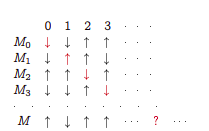
\includegraphics[scale=0.8]{tesi_stile/img/arresto.png}
\end{figure}
Se sapessi risolvere il problema dell’arresto, potrei costruire una macchina di Turing M che su ciascun input x si arresta se e solo se l’elemento x-esimo della diagonale è $\uparrow$.\\
Come prima, tale macchina non può comparire nella nostra tabella!\\
\textbf{Teorema}\\
Il problema dell’arresto non è decidibile.\\\\
\textbf{Dimostrazione}\\
Per assurdo supponiamo che H sia decidibile.\\
Allora anche il problema:
\begin{center}
    K = \{ x $\in$ N $|$ (x , x ) $\in$ H\}
\end{center}
è decidibile.\\
Invero, sia M una macchina di Turing che decide H. Il problema H è deciso dalla macchina M$'$ che esegue il seguente programma:\\
Su input x $\in$ $N$
\begin{center}
    \begin{enumerate}
        \item simula M su (x , x )
        
        \item restituisci l’output della computazione
    \end{enumerate}
\end{center}
\subsection{Il problema dell'arresto2}
Anche il complemento di K è decidibile e, di conseguenza semidecidibile. Più precisamente, K è accettato dalla macchina M$"$ che esegue il seguente programma.\\
Su input x $\in$ $N$
\begin{center}
    \begin{enumerate}
        \item Simula M su (x , x )
        
        \item Se l’output è NO, accetta; se l’output è SI, eseguire un loop infinito
    \end{enumerate}
\end{center}
Sia z l’indice della macchina M$"$. Allora\\
\begin{figure}[htp]
    \centering
    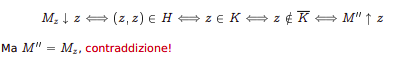
\includegraphics[scale=1]{tesi_stile/img/contraddizione.png}
\end{figure}
\subsection{Riduzioni}
Siano S e T due problemi. Una funzione totale e calcolabile $f$:$N$$\rightarrow$$N$ si dice riduzione del problema S al problema T se, per ogni x $\in$ N si ha:
\begin{center}
    x $\in$ S se e soltanto se $f(x)$ $\in$ T
\end{center}
\textbf{Proposizione}\\
Siano S e T due problemi. Se esite una riduzione di S a T e T è decidibile, allora S è decidibile.\\\\
\textbf{Dimostrazione}\\
Siano M e M$'$ rispettivamente la macchina di Turing che calcola f e quella che decide T. Allora S è deciso dalla macchina che esegue il seguente algoritmo.\\
Su input x
\begin{enumerate}
    \item simula M su x
    
    \item simula M$'$ sull’output di M
    
    \item restituisci l’output di M$'$
\end{enumerate}
\subsection{Riduzioni-2}
\textbf{Corollario}\\
Siano S e T due problemi. Se esite una riduzione di S a T e S è indecidibile, allora anche T è indecidibile.\\\\
\textbf{Proposizione}\\
Siano S e T due problemi. Se esite una riduzione di S a T e T è semidecidibile, allora S è semidecidibile.\\\\
\textbf{Esempio}\\
La funzione x $\in$ $N \mapsto (x,x)$ $\in$ $N^2$ è una riduzione del problema K al problema dell’arresto H.\\\\
\textbf{Osservazione}\\
Il problema dell’arresto è semi-decidibile.\\
Invero, è accettato dalla macchina di Turing universale.\\
\begin{center}
    Il problema\{(x,y, z) $\in$ $N^3$ $|$ M$_x$ $\downarrow$ y in al più z passi\}  \textbf{è decidibile}
\end{center}
\textbf{Teoria della programmazione}\\
Non è possibile costruire un sistema di debugging in grado di stabilire se un
programma termini o meno
\newpage
\subsection{Equivalenza di macchine di Turing}
\textbf{Problema dell’equivalenza di macchine di Turing}\\
Date due macchine di Turing, decidere se calcolano la medesima funzione:
\begin{center}
    E = \{(x , y) $|$ $\phi_x$ = $\phi_y$\}.
\end{center}
\textbf{Osservazione}\\
Due funzioni sono uguali se
\begin{itemize}
    \item hanno lo stesso dominio,
    
    \item hanno lo stesso valore su ogni elemento del dominio.
\end{itemize}
La dimostrazione richiede vari passi che utilizzano diagonalizzazione e riduzione
\newpage
\subsection{Funzioni Totali}
\textbf{Proposizione}\\
Il problema T = \{x $\in$ N $|$ $\phi_x$ è totale\} è indecidibile.\\\\
\textbf{Dimostrazione}\\
Per assurdo, sia T decidibile.\\
Allora c’è una funzione calcolabile totale f tale che T = f($N$).\\
Invero f è calcolata dal seguente algoritmo\\
\begin{figure}[htp]
    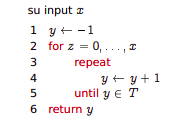
\includegraphics[scale=1]{tesi_stile/img/algo.png}
\end{figure}\\
La funzione g : $N$ $\mapsto$ $N$ definita da
\begin{center}
    g(x) = $\phi_f(x)$ (x)$+$1
\end{center}
è calcolabile totale. Pertanto, g = $\phi_f(z)$ per un opportuno z $\in$ $N$.\\
\begin{figure}[htp]
    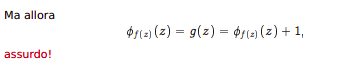
\includegraphics[scale=1]{tesi_stile/img/assurdo.png}
\end{figure}
\newpage
\subsection{Funzione Nulla}
La funzione nulla è la funzione calcolabile totale Z : x $\in$ N $\mapsto$ 0.\\\\
\textbf{Proposizione}\\
Per ogni x $\in$ N, consideriamo la funzione g$_x$ definita da:\\
\begin{figure}[htp]
    \centering
    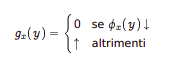
\includegraphics[scale=1]{tesi_stile/img/nulla.png}
\end{figure}\\
Si verifica facilmente che g$_x$ è calcolabile e anche il suo indice è calcolabile.\\
Invero esso è calcolato dal seguente algoritmo:\\
Su input x
\begin{center}
    \begin{enumerate}
        \item calcola il programma di M$_x$
        
        \item aggiungi al programma le istruzioni seguenti:
        \begin{itemize}
            \item se la macchina originale si arresta, output zero
        \end{itemize}
        \item restituisci il codice della macchina modificata
    \end{enumerate}
\end{center}
Quindi g$_x$ = $\phi_h(x)$, con h calcolabile totale. Inoltre\\
\begin{figure}[htp]
    \centering
    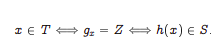
\includegraphics[scale=1]{tesi_stile/img/nulla2.png}
\end{figure}\\
Pertanto h è una riduzione di T a S.\\
Poiché T è indecidibile, lo sarà anche S.
\newpage
\subsection{Equivalenza di macchine di Turing}
\textbf{Proposizione}\\
Il problema E = \{(x , y) $\in$ $N^2$ $|$ $\phi_x$ = $\phi_y$\} è \textbf{indecidibile}\\\\
\textbf{Dimostrazione}\\
Sia z l’indice della funzione nulla.\\
La funzione f : x $\in$ N $\mapsto$ (x,z) $\in$ $N^2$ è una riduzione di S a E.\\
Poiché S è indecidibile, lo sarà anche E.\\\\
\textbf{Osservazione}\\
Non è possibile decidere se due generici programmi calcolano la stessa funzione: la correttezza semantica di un programma è indecidibile.






